\documentclass[titlepage,a4paper]{jsarticle}
\usepackage{../sty/import}% 各種パッケージインポート
\usepackage{../sty/title}% タイトルページの変更

%% タイトルページの変数
% レポートタイトル
\title{デザインパターン}
% 提出日
\expdate{\today}
% 科目名
\subject{オブジェクト指向プログラミング}
% 分野
\class{情報経営システム工学分野}
% 学年
\grade{B3}
% 学籍番号
\mynumber{24336488}
% 記述者
\author{本間 三暉}
% グループ名 % もし班があるやつならtitle_team.styを入れる
% \team{10}
\begin{document}
% titleページ作成
\maketitle
\section{デザインパターン}
% どのデザインパターンを選択したか記述すること
私はStateパターンを選択した.

Stateパターンは,オブジェクトが持つ状態によって異なる振る舞いを提供するためのデザインパターンである.
このパターンは,状態が変わることによってオブジェクトの動作が変化するシステムに適している.
Stateパターンを使用することで,状態遷移を明確にし,状態に依存するコードを整理することができる.
\subsection{どのようなところに応用できるか}
Stateパターンは以下のような場面で使えると考える.
\begin{itemize}
  \item ゲーム開発におけるキャラクターの動作管理
  \item GUIアプリケーションにおけるウィジェットの状態管理
  \item 通信プロトコルの実装における接続状態の管理
  \item ワークフローシステムにおけるタスクの進行状態の管理
\end{itemize}
\subsection{適用例}
% Stateパターンを適用する前のコードは,状態に依存する処理が複雑であり,メンテナンスが困難で.
% 例えば,状態によって異なる処理が行われるコードが存在した場合,状態が増えるにつれて条件分岐が増加し,コードが読みにくくなる.
図\ref{sub@適用前}にStateパターン適用前のNewCharacterを含むクラス図を示す.
また,図\ref{sub@適用後}にStateパターン適応後のNewCharacterを含むクラス図を示す.
\begin{figure}[H]
  \centering
  \begin{minipage}[]{0.8\hsize}
    \centering
    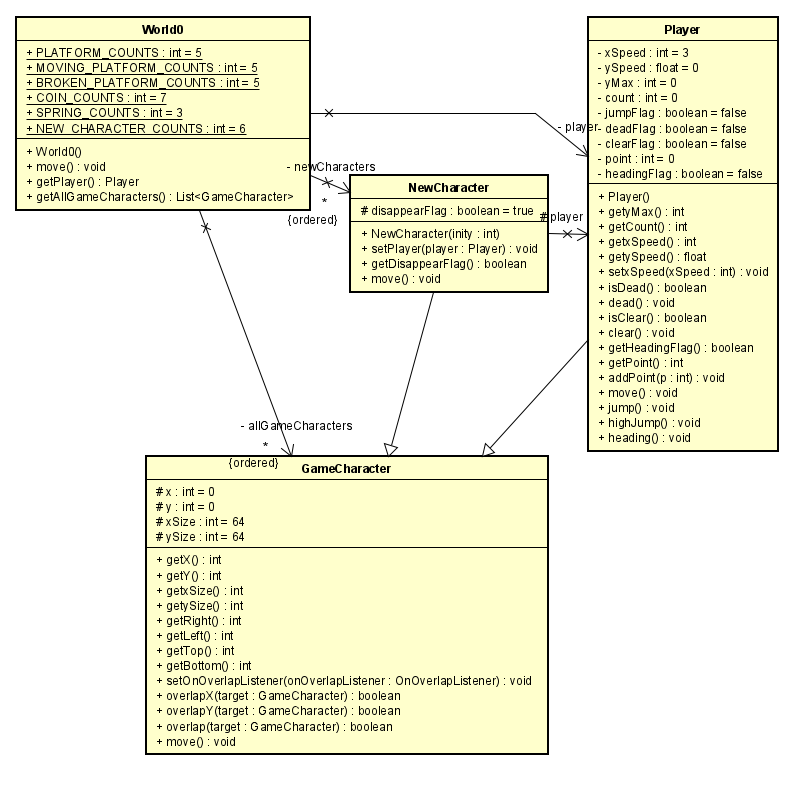
\includegraphics[width=7cm]{img/class.png}
    \subcaption{適用前}
    \label{適用前}
  \end{minipage}

  \begin{minipage}[]{0.8\hsize}
    \centering
    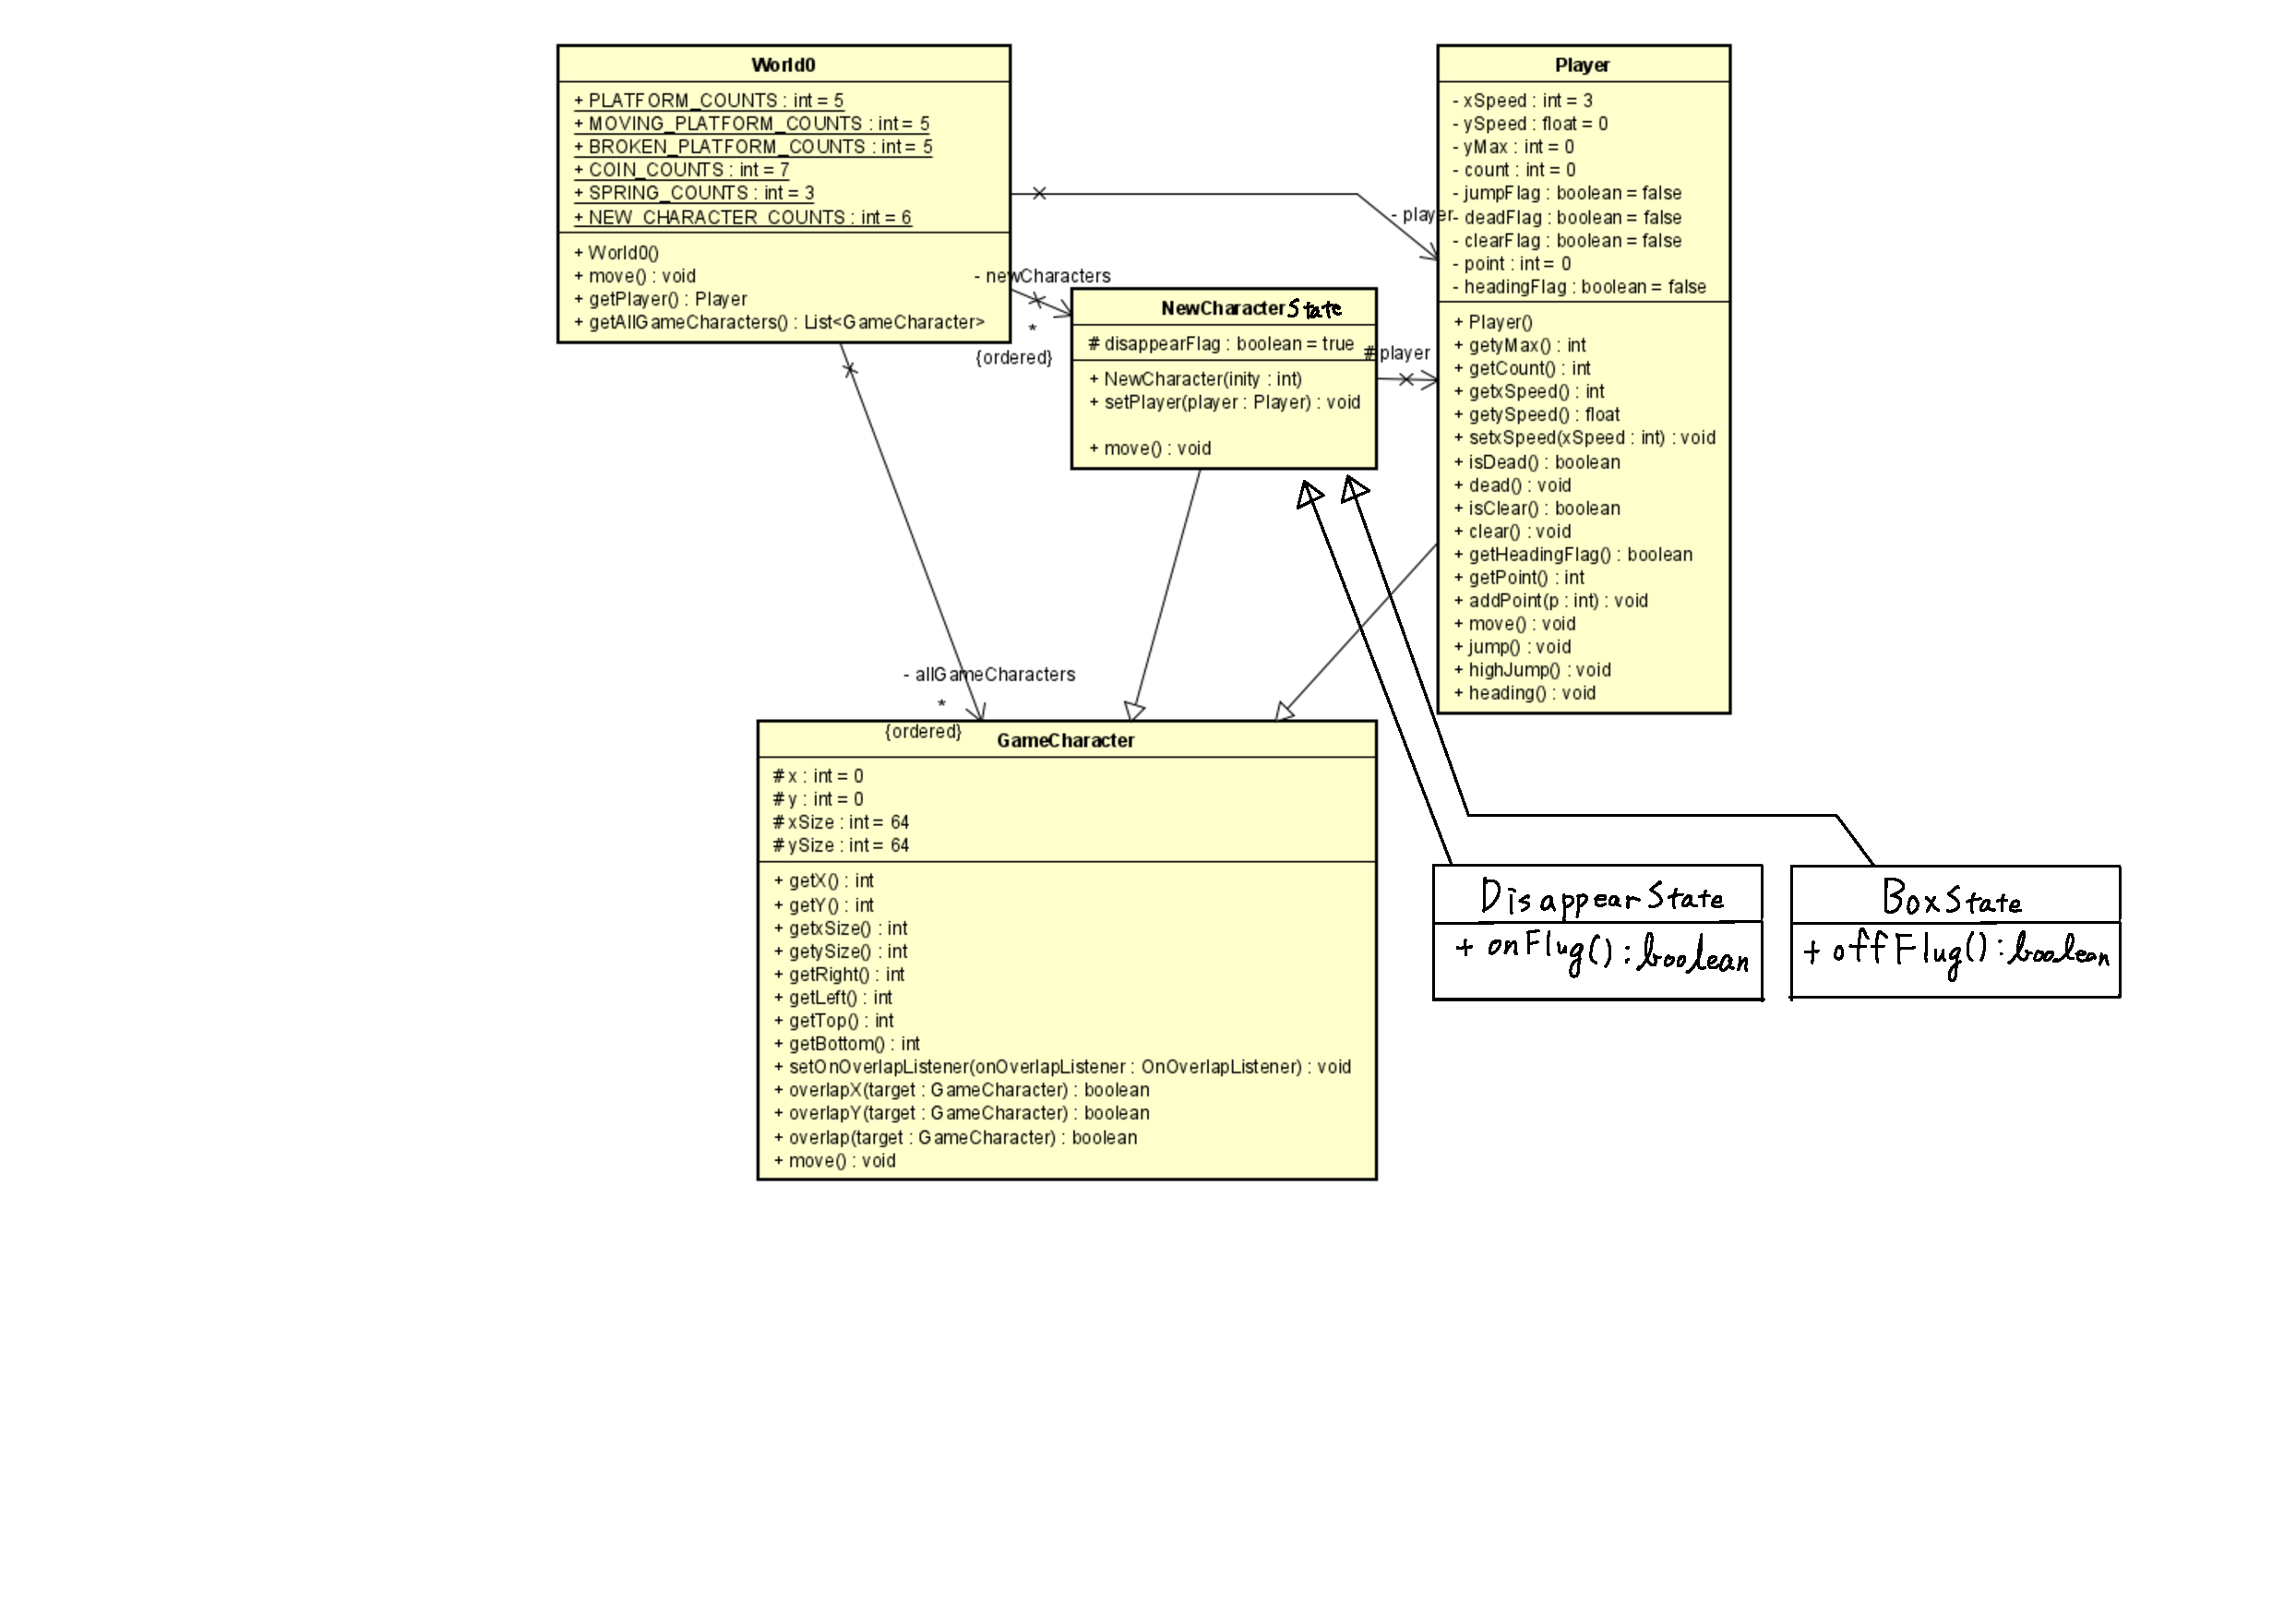
\includegraphics[width=10cm]{img/Class_After.pdf}
    \subcaption{適用後}
    \label{適用後}
  \end{minipage}
  \caption{デザインパターンの適用例}
  \label{デザインパターン}
\end{figure}
Stateパターンを適用すると,状態ごとの振る舞いを独立したクラスに分離することができる.
状態ごとの処理を分離することで,コードの可読性とメンテナンス性が向上する事がわかる.
\section{考察}
% ・デザインパターンの適用について、
% ・なぜこのパターンを選択したか?
% ・このパターンを適用することによるメリット
% ・このパターンを適用することによるデメリット
% 等について考察せよ。
Stateパターンを選択した理由は,状態遷移の複雑さを軽減し,状態ごとの振る舞いを分離することでコードの可読性と拡張性を向上させるためである.
状態遷移が明確になることで,バグの発見と修正が容易になる.
\subsection{メリット}
\begin{itemize}
  \item 可読性の向上: 状態ごとの振る舞いが独立したクラスに分離されるため,コードが読みやすくなる.
  \item 拡張性の向上: 新しい状態を追加する際に,既存のコードを変更する必要が少なくなる.
  \item メンテナンス性の向上: 状態ごとの処理が独立しているため,バグの発見と修正が容易になる.
\end{itemize}
\subsection{デメリット}
\begin{itemize}
  \item クラスの増加: 状態ごとにクラスを定義するため,クラスの数が増加する.
  \item 複雑さの増加: 状態遷移の管理が複雑になる場合がある.
\end{itemize}

\section{感想}
% ※ここは採点の対象外です。
% 今回の実験の内容について感想などあれば記述して下さい。
% 次年度以降の実験の実施に役立てたいと思います。
Stateパターンを学ぶことで,オブジェクト指向プログラミングの設計原則を深く理解することができた.
状態ごとの振る舞いを明確にすることで,コードの品質を向上させることができると感じた.
次年度以降も,このようなデザインパターンの学習を通じて,より良いソフトウェア設計を目指していきたいと思う.
\end{document}
